\section{Experimental Protocol}
\label{sec:experimental_protocol}

The experimental protocol is designed to evaluate held-out in-domain performance and independent cross-dataset generalization while preventing model-selection leakage. LOL-v1 is handled separately as a deliberately non-independent overlap-control set and is excluded from the independent-generalization interpretation. All models are trained on a single source domain, LOL-v2 Real, and the validation split is used for early stopping, checkpoint selection, and model selection. The test sets are never used during these steps and are evaluated only after the final configuration has been selected.

The project is organized around model families. For each family, a dedicated grid search explores meaningful architectural and optimization choices, while the other parts of the experimental procedure are kept unchanged whenever possible. These common parts include the data augmentation policy, the training and validation procedure, and the validation-based selection strategy. In this way, different model families can be compared under consistent experimental conditions and under a similar computational budget.

Across comparable runs, the training setup keeps fixed the batch size, the data-loading strategy, the validation frequency, the use of mixed precision when supported by the hardware, and the choice of favoring efficiency over fully deterministic execution. The maximum number of training epochs is intentionally set as a large upper bound, because the effective training duration is controlled by early stopping rather than by a fixed epoch budget.

Early stopping is implemented in a model-agnostic way. The monitored validation metric, its optimization direction, and the optional tie-breaker metric can be selected according to the specific experiment or model family. However, the overall early-stopping policy is kept fixed across comparable runs, so that all configurations are selected according to the same validation-based logic.

For each model family, the experimental protocol consists of four stages: (i) a screening stage, in which all grid-search configurations are trained with a fixed seed and ranked by validation performance; (ii) a multi-seed re-training stage, in which the most promising configurations are re-trained with multiple random seeds to estimate performance and stability; (iii) a validation-based model-selection stage, in which the final configuration is chosen from aggregated multi-seed validation results; and (iv) a final evaluation stage, in which the selected configuration is tested on LOL-v2 Real, LOL-v2 Synthetic, MILLs, and ExDark. LOL-v1 is evaluated separately as an overlap-control diagnostic. Test evaluation is disabled during screening and model selection and enabled only in the final evaluation stage. Figure~\ref{fig:experimental_protocol} provides a visual overview of this workflow.

\begin{figure*}[t]
    \centering
    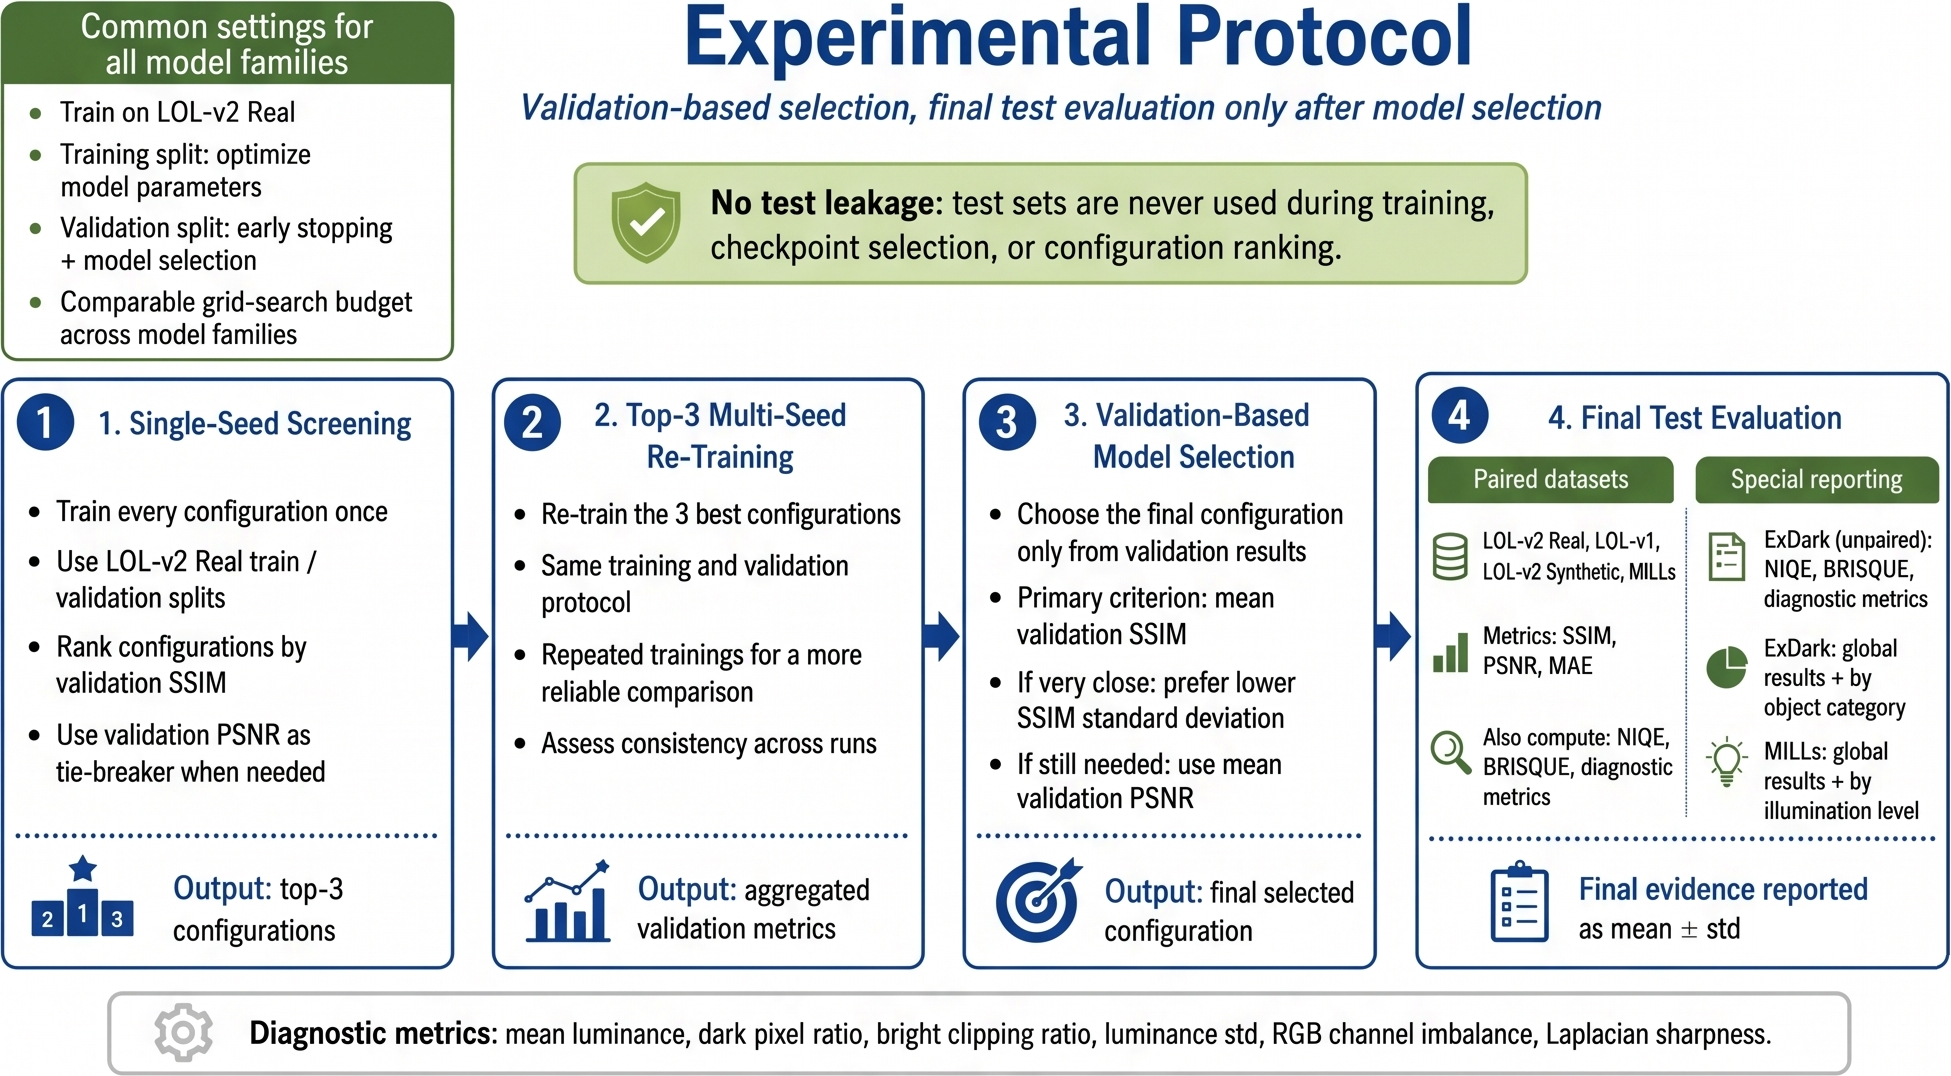
\includegraphics[width=\textwidth]{fig/experimental_protocol/experimental_protocol.png}
    \caption{Overview of the experimental protocol. Held-out in-domain test evidence is obtained from LOL-v2 Real, while independent external test evidence is obtained from LOL-v2 Synthetic, MILLs, and ExDark. LOL-v1 is evaluated separately as a non-independent overlap-control set.}
    \label{fig:experimental_protocol}
\end{figure*}

\subsection{Single-Seed Screening}

The first experimental stage is a single-seed grid search, in which every configuration is trained using a single fixed seed. The purpose of this stage is not to produce final evidence, because a single seed can be affected by random initialization and data-loader randomness. Instead, the purpose is to reduce the search space and identify a small number of promising configurations.

All configurations are trained on the LOL-v2 Real training split and monitored on the LOL-v2 Real validation split; test sets are not evaluated during screening. For each run, checkpoints are selected primarily by validation SSIM~\cite{DBLP:journals/tip/WangBSS04}, as low-light enhancement should preserve structural similarity to the reference image, including luminance, contrast, and local structure rather than merely minimize average pixel-wise error. Validation PSNR, a logarithmic measure of pixel-wise reconstruction quality, is also computed and used as a tie-breaker: when validation SSIM values fall within the configured tolerance, the checkpoint with the higher PSNR is selected.

The output of this stage is a validation-based ranking of the explored configurations. This ranking is later parsed from the run logs and used to select the top-3 configurations for the multi-seed stage.

\subsection{Top-3 Multi-Seed Re-Training}

After the screening stage, the three most promising configurations are selected from the validation-based ranking and re-trained under the same training and validation protocol. This stage is necessary because the screening phase provides only a preliminary estimate of performance, obtained from a single training run for each configuration.

The goal of the multi-seed stage is to obtain a more reliable comparison among the selected configurations. By repeating the training procedure several times for each of them, the protocol can evaluate whether its validation performance is consistent or mainly due to a favorable run.

The outputs of this stage are aggregated validation metrics for each selected configuration. These aggregated results are then used for the final validation-based selection, while the test sets remain untouched.

\subsection{Validation-Based Model Selection}

The final configuration is selected only from the aggregated validation results of the multi-seed stage.

The primary criterion is mean validation SSIM across runs. For very close mean SSIM values, the more stable configuration is favored, based on validation SSIM standard deviation. If still ambiguous, mean validation PSNR is the final tie-breaker.

This rule keeps the whole selection process validation-based, while also accounting for statistical robustness across repeated trainings.

\subsection{Final Test Evaluation}

Final test evaluation is performed only after the final configuration has been selected. The selected configuration is then evaluated on the test sets of all datasets, and the resulting metrics are aggregated as mean and standard deviation. This ensures that the final evidence reflects both average performance and statistical robustness across repeated runs.

The evaluation protocol depends on whether a dataset is paired or unpaired. For paired datasets, ``full-reference'' metrics are computed by comparing the enhanced model output with the corresponding target image. In this work, paired datasets are evaluated using SSIM, PSNR, and mean absolute error (MAE), which measures the average absolute pixel difference between the enhanced and reference images.

``No-reference'' metrics do not require target images and are computed for both paired and unpaired datasets. The metrics used are naturalness image quality evaluator (NIQE)~\cite{DBLP:journals/spl/MittalSB13}, which measures the deviation from statistical properties commonly found in natural images, and blind/referenceless image spatial quality evaluator (BRISQUE)~\cite{DBLP:journals/tip/MittalMB12}, which estimates perceptual quality from spatial scene statistics.

Additional diagnostic metrics are computed on model outputs for both paired and unpaired datasets to support the interpretation of failure modes, i.e., recurring enhancement errors. These include: (i) mean luminance, measuring average brightness; (ii) dark pixel ratio, measuring the fraction of pixels that remain very dark; (iii) bright clipping ratio, measuring the fraction of near-saturated pixels; (iv) luminance standard deviation, providing an indication of contrast variation; (v) red-green-blue (RGB) channel imbalance, helping detect color cast; and (vi) Laplacian sharpness, providing a simple estimate of high-frequency content related to blur, noise, or halo artifacts.

LOL-v2 Real, LOL-v2 Synthetic, and MILLs are paired datasets and are evaluated using full-reference, no-reference, and diagnostic output metrics. MILLs is additionally reported both globally across all samples and separately by illumination level. This grouped reporting is useful because MILLs contains inputs captured under different illumination conditions, allowing an analysis of how performance varies with illumination.

ExDark is unpaired and does not provide normally exposed target images. It is therefore evaluated only with no-reference and diagnostic output metrics. In addition to global results over the full dataset, ExDark is analyzed by object category, since its images are organized into semantic groups.

LOL-v1 is paired, but its full-reference, no-reference, and diagnostic results are reported only as descriptive overlap-control results because it overlaps with LOL-v2 Real.